\documentclass[tikz,border=8pt,multi=tikzpicture]{standalone}
\usepackage{amsmath}
\usepackage{xcolor}
\usetikzlibrary{arrows.meta, calc}

\definecolor{mainblue}{HTML}{001158}
\definecolor{accent}{HTML}{8592bc}
\definecolor{lightaccent}{HTML}{e7e9f2}

\tikzset{
  force/.style={-{Stealth[length=3mm]}, line width=1.2pt, color=mainblue},
  dim/.style={-{Stealth[length=2mm]}, line width=0.7pt, color=accent},
  axis/.style={-{Stealth[length=2mm]}, line width=0.6pt, color=black!45, dashed},
  every node/.append style={font=\sffamily}
}

\begin{document}

% ---------- Figure: block on incline, force parallel to slope, angle alpha ----------
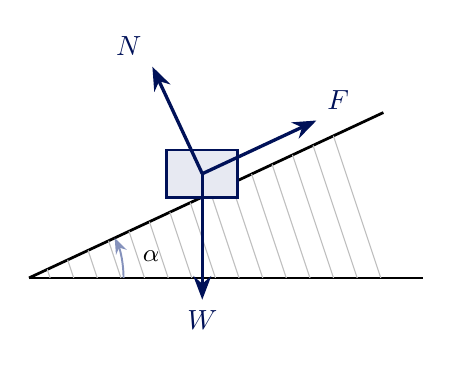
\begin{tikzpicture}
\draw[line width=1pt] (0,0) -- (5,0);
\draw[line width=1pt] (0,0) -- (4.5,2.1);
\draw[dim] (1.2,0) arc (0:25:1.2);
\node at (1.55,0.28) {\small $\alpha$};
\begin{scope}
  \clip (0,0) -- (4.5,2.1) -- (5,0) -- cycle;
  \foreach \x in {0,0.3,...,5} {\draw[gray!50, line width=0.4pt] (\x,-1) -- (\x-1,2);}
\end{scope}
\coordinate (P) at (2.3,1.073);
\fill[lightaccent, draw=mainblue, line width=1pt] ($(P)+(-0.55,-0.05)$) rectangle ++(0.9,0.6);
\coordinate (Ctr) at ($(P)+(-0.1,0.25)$);
\draw[force] (Ctr) -- ++(0,-1.6) node[below] {$W$};
\draw[force] (Ctr) -- ++(115:1.5) node[above left] {$N$};
\draw[force] (Ctr) -- ++(25:1.6) node[above right] {$F$};
\end{tikzpicture}

% ---------- Figure: five forces, angles from different reference axes ----------
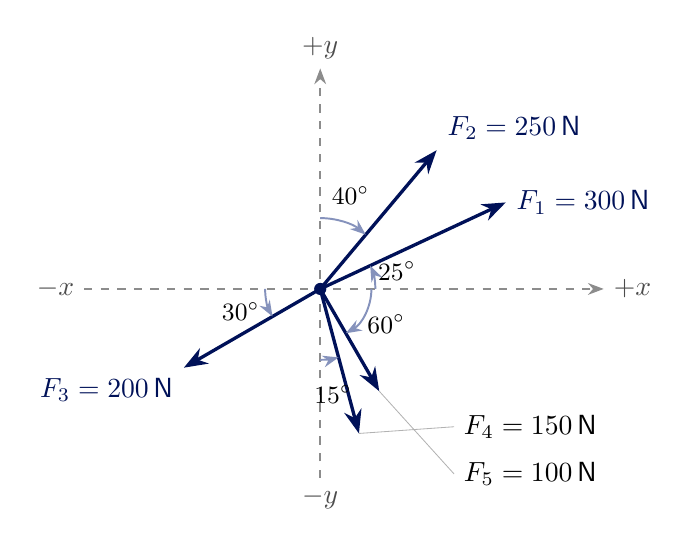
\begin{tikzpicture}
\coordinate (O) at (0,0);
\draw[axis] (-3.0,0) -- (3.6,0) node[right, color=black!70] {$+x$};
\node[left, color=black!70] at (-3.0,0) {$-x$};
\draw[axis] (0,-2.4) -- (0,2.8) node[above, color=black!70] {$+y$};
\node[below, color=black!70] at (0,-2.4) {$-y$};
\fill[mainblue] (O) circle (2.2pt);

\draw[force] (O) -- (25:2.6) node[right] {$F_1=300\,\text{N}$};
\draw[dim] (0.7,0) arc (0:25:0.7);
\node at (13:1.0) {\small $25^\circ$};

\draw[force] (O) -- (50:2.3) node[above right] {$F_2=250\,\text{N}$};
\draw[dim] (90:0.9) arc (90:50:0.9);
\node at (72:1.25) {\small $40^\circ$};

\draw[force] (O) -- (210:2.0) node[below left] {$F_3=200\,\text{N}$};
\draw[dim] (180:0.7) arc (180:210:0.7);
\node at (196:1.05) {\small $30^\circ$};

\draw[force] (O) -- (285:1.9);
\draw[gray!60, line width=0.3pt] (285:1.9) -- (1.7,-1.75);
\node[anchor=west] at (1.7,-1.75) {$F_4=150\,\text{N}$};
\draw[dim] (270:0.9) arc (270:285:0.9);
\node at (277:1.35) {\small $15^\circ$};

\draw[force] (O) -- (300:1.5);
\draw[gray!60, line width=0.3pt] (300:1.5) -- (1.7,-2.35);
\node[anchor=west] at (1.7,-2.35) {$F_5=100\,\text{N}$};
\draw[dim] (360:0.65) arc (360:300:0.65);
\node at (332:0.95) {\small $60^\circ$};

\end{tikzpicture}

\end{document}
